\documentclass[a4paper,11pt]{article}

\usepackage[T1]{fontenc}
\usepackage[utf8]{inputenc}
\usepackage{graphicx}
\usepackage{xcolor}
\usepackage{float}
\usepackage{hyperref}
\usepackage{amsmath,amssymb,amsthm,textcomp}
\usepackage{enumerate}
\usepackage{multicol}
\usepackage{tikz}
\usepackage{geometry}
\usepackage{subcaption}
\usepackage{multirow}
\usepackage{array}

\geometry{
left=25mm,right=25mm,%
bindingoffset=0mm, top=20mm,bottom=20mm}

\hypersetup{
    bookmarksnumbered=true,
    bookmarksopen=false,
    bookmarksopenlevel=1,
    colorlinks=false,
    pdfstartview=Fit,
    pdfpagemode=UseOutlines,
    pdfpagelayout=TwoPageRight,
    pdfborder = {0 0 0}
}

\newcommand{\figur}[5][0]{
		\begin{figure}[H] \centering \em %H / h!
			\includegraphics[width=#5\textwidth, angle=#1]{#2}
			\caption{#3}\label{fig:#4}
		\end{figure}
}

\linespread{1.3}

\newcommand{\linia}{\rule{\linewidth}{0.5pt}}

\newcolumntype{C}[1]{>{\centering}m{#1}}


% my own titles
\makeatletter
\renewcommand{\maketitle}{
\begin{center}
\vspace{2ex}
{\huge \textsc{\@title}}
\vspace{1ex}
\\
\linia\\
\@author \hfill  \studyno
\vspace{4ex}
\end{center}
}
\makeatother
%%%

% custom footers and headers
\usepackage{fancyhdr,lastpage}
\pagestyle{fancy}
\lhead{}
\chead{}
\rhead{}
\lfoot{\handindate}
\cfoot{}
\rfoot{Page \thepage\ /\ \pageref*{LastPage}}
\renewcommand{\headrulewidth}{0pt}
\renewcommand{\footrulewidth}{0pt}

\hbadness=10001
\hfuzz=1000pt

\begin{document}

\title{CTA200H: Projet}
\author{Andoni Torres}
\def\studyno{18/05/2018}

\maketitle

\section{Summary}

The code reads three data files containing various parameters related to numerical relativity simulations of neutron star mergers with different total masses. The files contain a different amount of columns.

First, all data is imported and the linear correlation is evaluated. If the correlation coefficient is sufficient, the data is then plotted. We find 18 pairs of data with a coeff. above 0.95 out of a total of 45 pairs. Notably, \textit{dominant post merger frequency}  and all radius data, \textit{f-mode post-merger frequency} and all radius data and \textit{spiral port-merger frequency} with r12, r125 and r16 (not rmax).

The code then focuses on the correlation between parameters \textit{f-mode post-merger frequency} and radius of a 1.6 M$_\odot$ neutron star. 

The data is fitted to a linear model using Markov chain Monte-Carlo algorithm (MCMC). The slope and intercept are evaluated. The plotted data is shown in graph \ref{im2}.

After, the same steps are repeated, this time with a quadratic model. Graph \ref{im3} shows the output.

Finally, all  \textit{f-mode post-merger frequency} and radius of a 1.6 M$_\odot$ neutron star data is imported from the three files and fitted to a linear model. This results in significantly different parameters but an uncertainty of the same order of magnitude.

Table \ref{tab:param} shows all results.

The equation below is used to calculate all plotted uncertainties using the output $\delta x_i$ from the fitting.

\begin{equation*}
    \Delta f(x_i) = \sqrt{ \sum_i \left( \frac{\partial f(x_i)}{\partial x_i} \cdot \delta x_i\right)^2}
    \label{eq1}
\end{equation*}


\section{Results}
\begin{figure} [h]
    \centering
    \begin{subfigure}[b]{0.45\textwidth}
        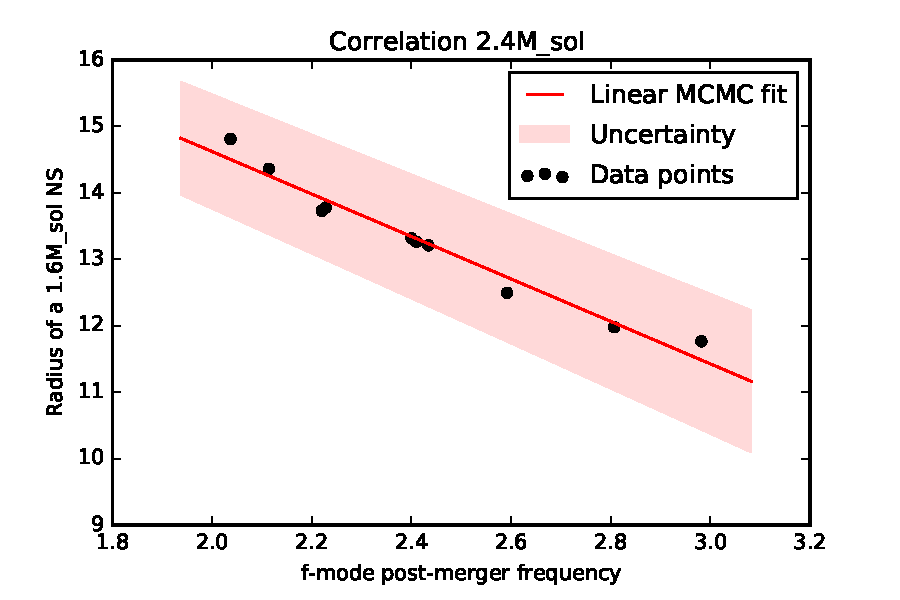
\includegraphics[width=\textwidth]{linear_fit.pdf}
        \caption{Model: Linear. Data set: 2.4$_{\odot}$}
        \label{im2}
    \end{subfigure} 
    \begin{subfigure}[b]{0.45\textwidth}
        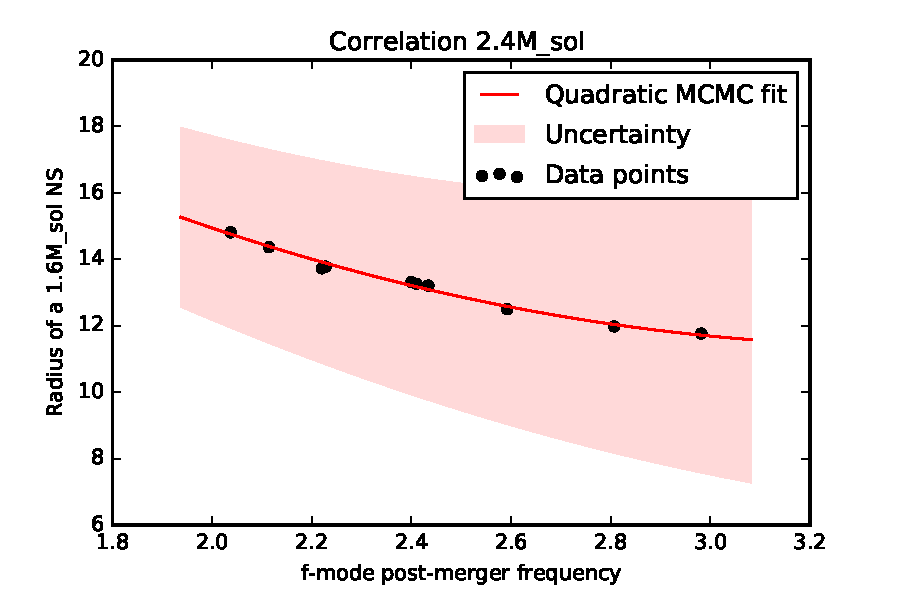
\includegraphics[width=\textwidth]{quadratic_fit.pdf}
        \caption{Model: Quadratic. Data set: 2.4$_{\odot}$}
        \label{im3}
    \end{subfigure} 
    \begin{subfigure}[b]{0.45\textwidth}
        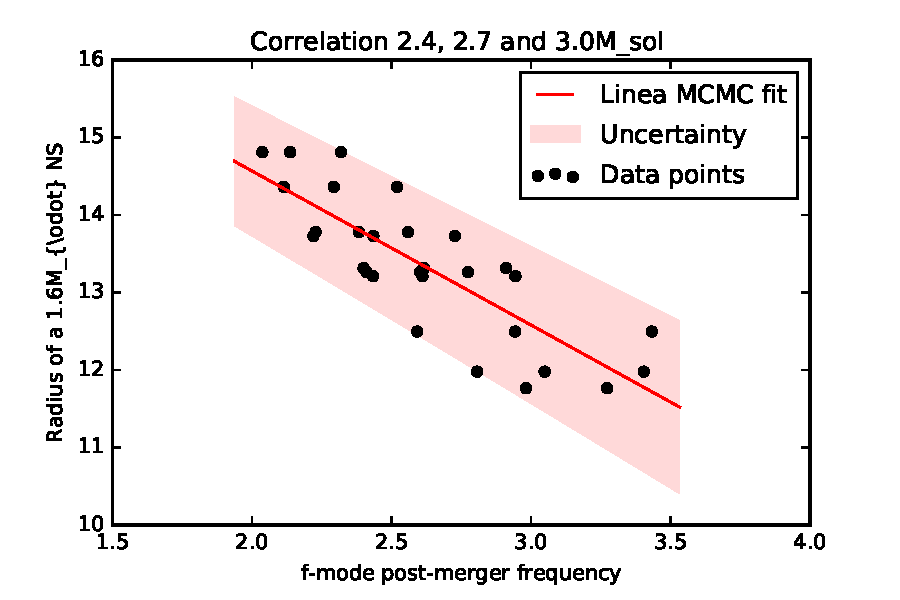
\includegraphics[width=\textwidth]{linear_all3.pdf}
        \caption{Model: Linear. Data set: 2.4, 27 and 3.0M$_{\odot}$}
        \label{im4}
    \end{subfigure}
    \caption{Markov Chain Monte-Carlo fit and uncertainty zone with different models and data sets.}
    \label{im5}
\end{figure}

\begin{table}[h]
    \caption{Parameters.}
    \centering
    \begin{tabular}{c | c |  C{2cm} |c |c | c }
    \hline
    Data Set & N steps & Acceptance ratio & Model & Équation & Parameters \\
    \hline
    \hline
\multirow{3}{*}{$2.4 M_\odot$} & \multirow{4}{*}{100000} &	0.32 & Linear	&$m\cdot x + b$ & $m = -3.18 \pm 0.27$, $b=20.98\pm0.68$\\
&	& \multirow{2}{*}{0.13}	& \multirow{2}{*}{Quadratic} & \multirow{2}{*}{$ax^2+b+c$}  & $a = 1.76 \pm 0.25$, $b = -12.01 \pm 1.16$\\
&&&&&$c = 31.93 \pm 1.60$\\\
$2.4, 2.7, 3.0 M_\odot$	&		&	0.20	& Linear	&$m\cdot x + b$ & $ m = -2.01 \pm 0.25$, $
b = 18.59 \pm 0.67$\\
    \hline
    \end{tabular}
\label{tab:param}
\end{table}

\end{document}